\documentclass[12pt,a4paper]{article}
\usepackage{graphicx}
\usepackage{graphics}
\usepackage{listings}
\usepackage{caption}
\usepackage{courier}
\usepackage{color}
\usepackage{xcolor}

\lstset{
    basicstyle=\footnotesize\ttfamily,
    numberstyle=\tiny,
    numbersep=5pt,
    tabsize=2,
    extendedchars=true,
    breaklines=true,
    keywordstyle=\color{red},
        frame=b,
    stringstyle=\color{white}\ttfamily,
    showspaces=false,
    showtabs=false,
    xleftmargin=17pt,
    framexleftmargin=17pt,
    framexrightmargin=5pt,
    framexbottommargin=4pt,
    showstringspaces=false
}
\lstloadlanguages{C}

\DeclareCaptionFont{white}{\color{white}}
\DeclareCaptionFormat{listing}{
    \colorbox[cmyk]{0.43, 0.35, 0.35, 0.01}{
        \parbox{\textwidth}{\hspace{15pt}#1#2#3}
    }
}
\captionsetup[lstlisting]{
    format=listing,
    labelfont=white,
    textfont=white,
    singlelinecheck=false,
    margin=0pt,
    font={bf,footnotesize}
}

\newcommand{\doctitle}{%
Sculptural Illustration of Algorithms}

\pagestyle{myheadings}
\markboth{\hfill\doctitle}{\doctitle\hfill}

\bibliographystyle{siam}

%\addtolength{\textwidth}{1.00in}
%\addtolength{\textheight}{1.00in}
%\addtolength{\evensidemargin}{-1.00in}
%\addtolength{\oddsidemargin}{-0.00in}
%\addtolength{\topmargin}{-.50in}

\hyphenation{in-de-pen-dent}

\title{\textbf{\doctitle}\\
Independent Study Project Proposal}

\author{David E. Shere}

\begin{document}

\thispagestyle{empty}

\maketitle

My intention with this project is to build at least one sculpture in a series
with the purpose of artistically illustrating the operation of various sorting
algorithms\cite{wiki:sorting_algorithm}.  The sculptures will be constructed out
of either wood or a plastic and will use lighting acrylic on top of high power
LEDs to illustrate the sorting algorithms, which will be implemented on
microcontrollers powering the LEDs.  The two main objectives of this project
will be to explore the areas where technology and art meet, and secondarily to
improve my skills at using tools such as table and chop saws to construct
objects.  Michael McGinnis would be my supporting instructor and provide
feedback and input about my progress and ideas.  I will meet with him on
Wednesdays from 1PM to 4PM weekly.  On occasion, I might meet instead from 9AM to
12PM or on Mondays if there is a reason that would work better.

\subsection*{Exploring the Boundaries of Technology and Art}

The primary objective of this project will be to spend time investigating the
use of technology in creating sculptural works of art.  This project will
require the use of both computer engineering and artistic skills.  The computer
engineering side will involve the understanding of the algorithms that will be
illustrated and the ability to build the software that will power the
illustration.  The artistic side will be exercised by the aesthetic decisions in
terms of the display of the algorithm, and by the skill required to build a well
constructed sculpture.

Most of the technological parts of this project will be done at home where I
have the parts and equipment necessary to build the required circuit.  Ideally I
would use tricolor RGB (Red Green Blue) LEDs in order to use a wide variety of
colors but if I cannot afford to buy them I will use two colored LEDs instead
and simply create a gradient between the two colors.  A
microcontroller will have a collection of different colors
randomize, and step by step sort them into order.  In the case of the colors red,
yellow, green, and blue, it may start with the ordering "Blue, Red, Green,
Yellow," and then step by step rearrange the colors until they are in the proper
spectral order of "Red, Yellow, Green, Blue."  If I use two color LEDs it will
instead sort itself into a gradation between the two colors, such as a
continuation from blue to red with shades of violet forming the middle values.

The sculptural aspect of this work will be in determining the best way to
present this sorting.  My current idea is to create a long, segmented box
divided into spaces that will each contain a single LED (see figure
\ref{fig:diagram}).  Above each box will be a smaller rectangular box containing
a single white LED that will indicate which position the computer is currently
sorting.  The result will be a kinetic sculpture that gradually moves from a
random initial state to an ordered final state.

\subsection*{Gaining Experience with Construction Equipment}

Though the main objective for this project it to learn more about incorporating
technology and art together another motivation is to gain more experience using
the tools available in the sculpture workshop.  While taking Intermediate and
Advanced Sculpture I used the table and chop saws a great deal when working on
my projects.  While I have a fairly solid understanding of how to use these
tools I feel I could stand to get more comfortable with them.  Working on this
project would give me the opportunity to learn more about their effective use
including the use of specialized jigs and fixtures.

\subsection*{Evaluation of Work}

The way I plan to work on this project is by doing most of the technological
work at home and doing the actual building of the visible sculpture on campus.
The first half of the semester would probably be mostly spent developing the
software and electronics that would power the sculpture while evaluating
possible arrangements of the lights with maquettes.  At mid-semester I should
have a fairly complete design for the software, electronics, and the sculpture's
actual form.  The second half of the semester would be spend building the actual
piece or pieces.  Throughout the semester I would be meeting with Michael
McGinnis for his input and expertise.  The project will be graded in a verbal
critique of the work with Michael McGinnis at midterm and finals week and he
will also assign a written grade.

\bibliography{statement}

\pagebreak
\begin{figure}[here]
    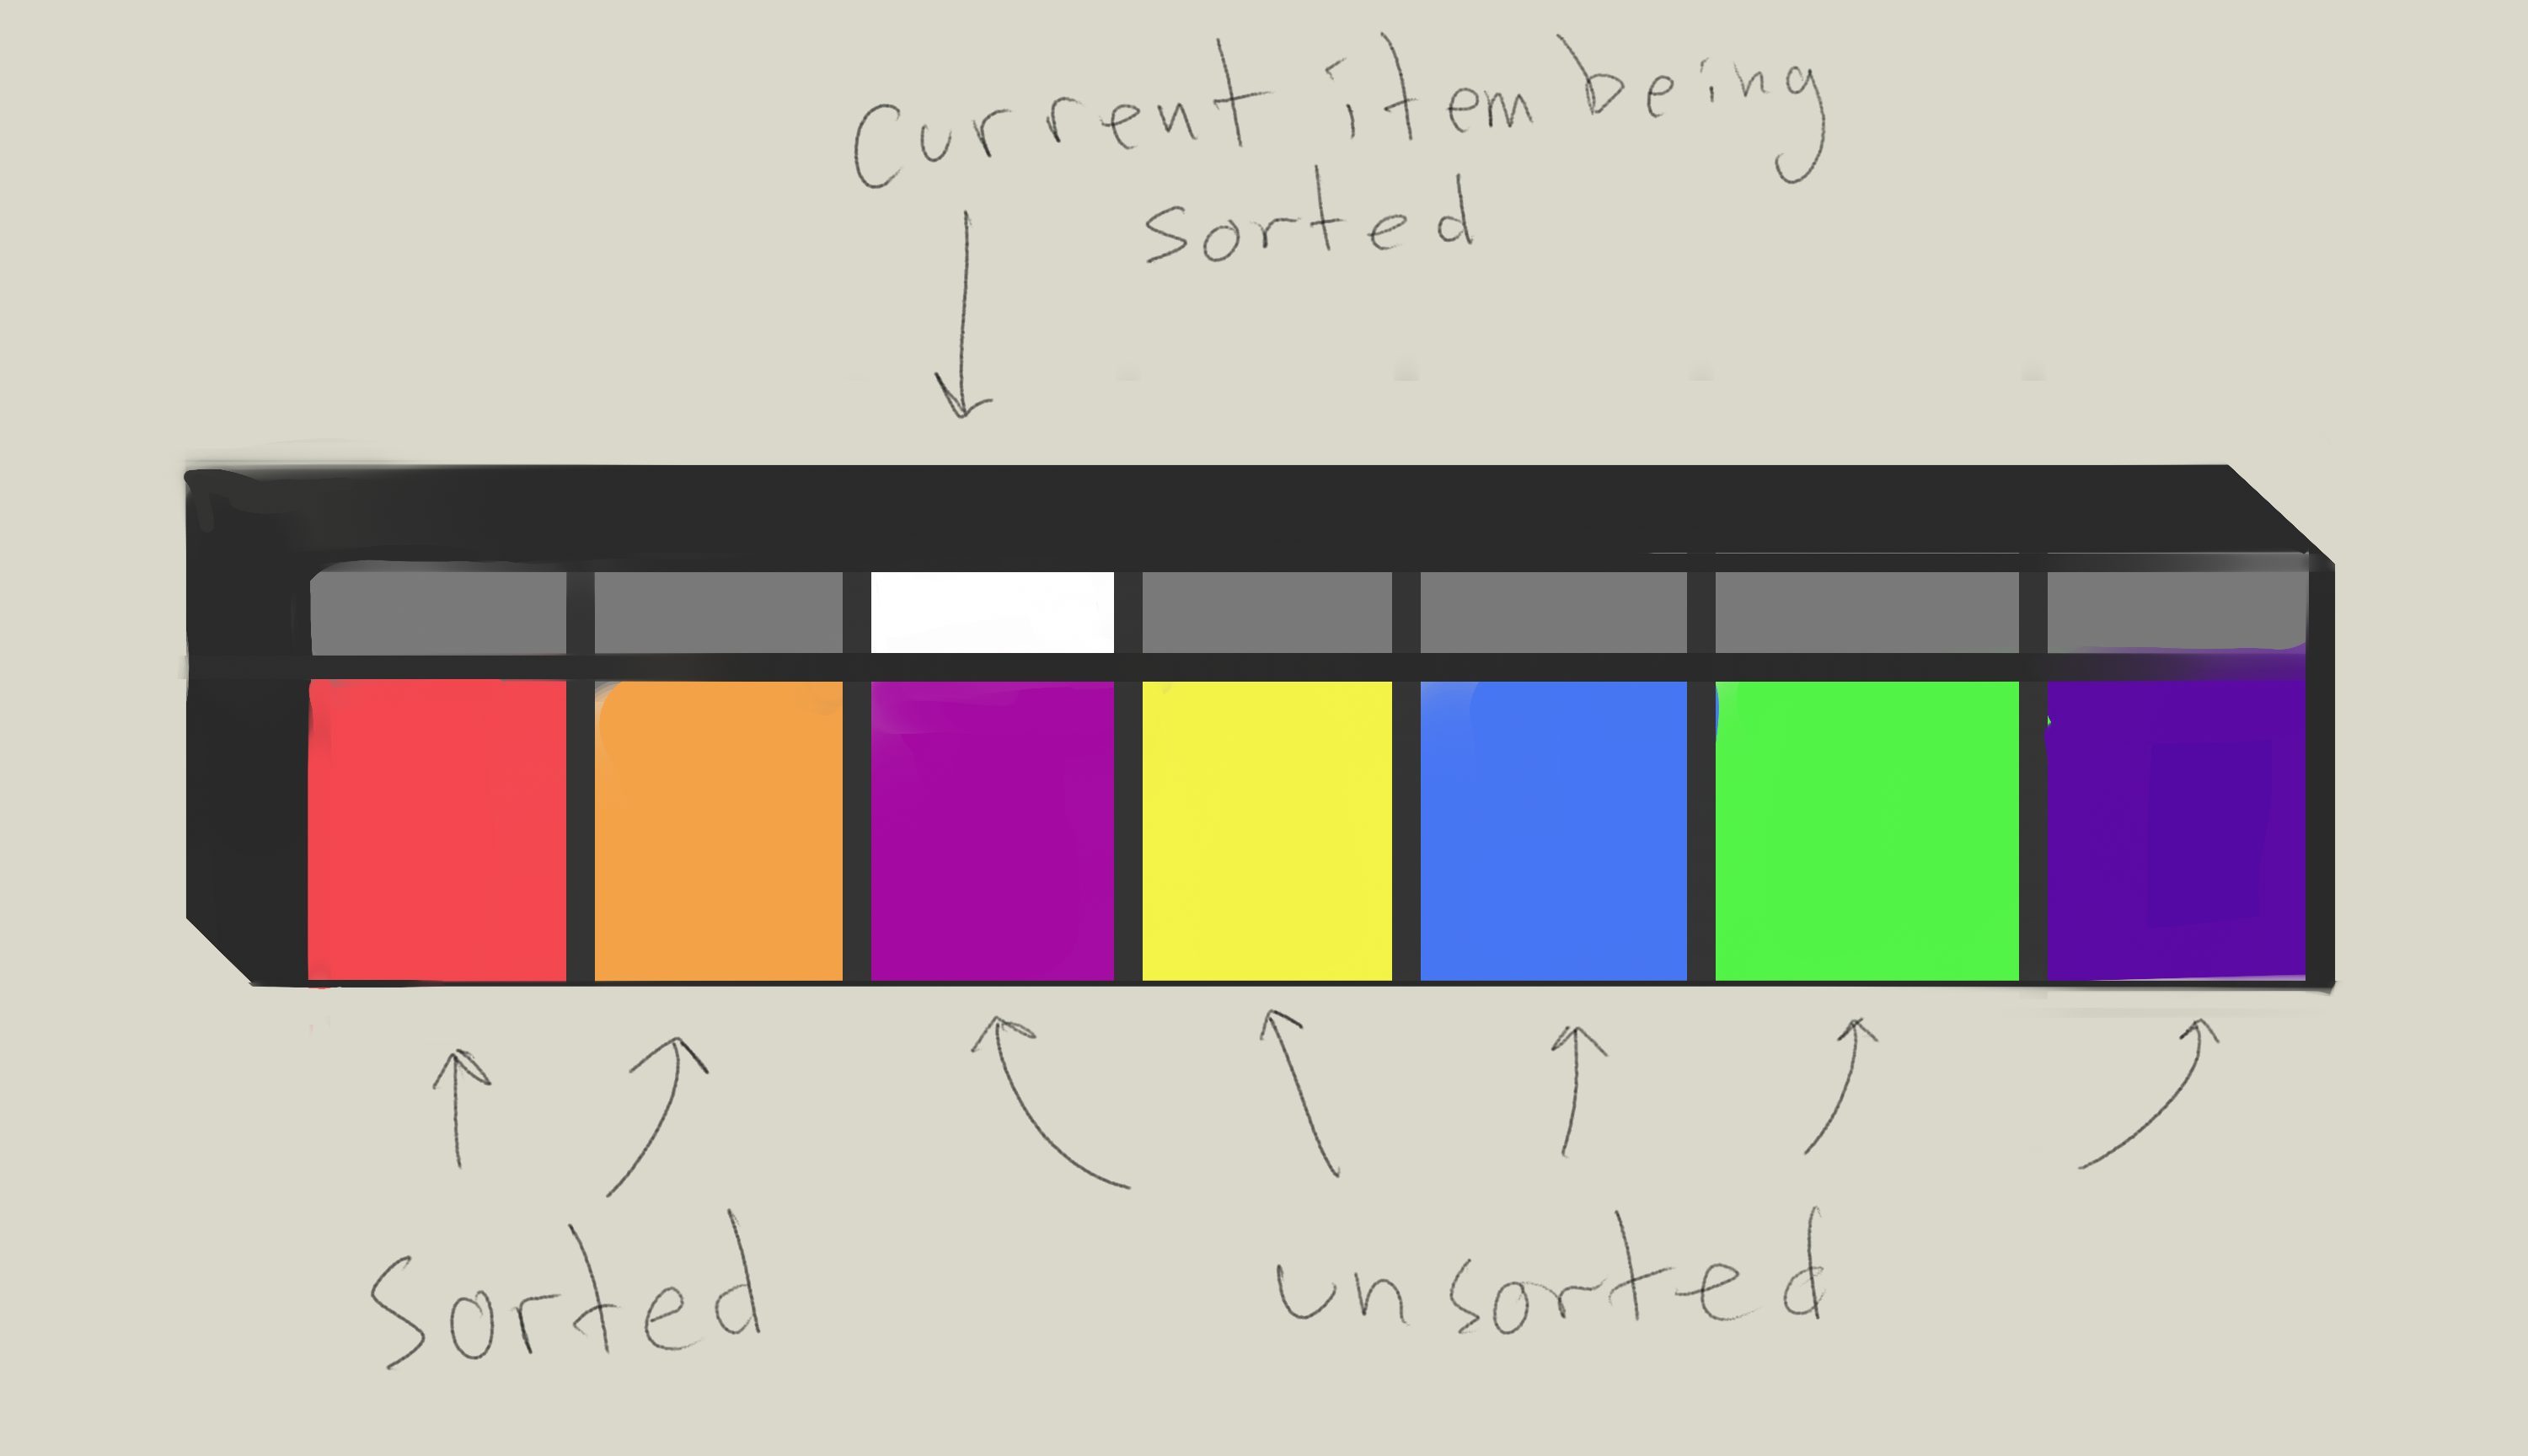
\includegraphics[width=0.9\textwidth]{images/diagram.png}
    \caption{Diagram of a possible manifestation of one sculpture in the series.}
    \label{fig:diagram}
\end{figure}

\pagebreak
\lstinputlisting[label=main.c, caption=main.c]{../src/main.c}

\pagebreak
\lstinputlisting[label=sort.h, caption=sort.h]{../src/sort.h}

\pagebreak
\lstinputlisting[label=sort.c, caption=sort.c]{../src/sort.c}

\pagebreak
\lstinputlisting[label=shift.h, caption=shift.h]{../src/shift.h}

\pagebreak
\lstinputlisting[label=shift.c, caption=shift.c]{../src/shift.c}

\end{document}
